\documentclass[a4paper]{article}

\usepackage[portuguese]{babel}
\usepackage[utf8]{inputenc}
\usepackage[T1]{fontenc}
\usepackage{algorithmic}
\usepackage{algorithm}
\usepackage{graphicx}
\usepackage{caption}
\usepackage{anysize}
\usepackage{amsmath}

\usepackage{hyperref}
\hypersetup{
	pdftitle = {[CAD] TP2: Parallel Programming for Clusters using MPI}
	,pdfauthor = {João Ferreira \& José Ribeiro\\ Departamento de Engenharia Informática\\ Universidade De Coimbra\\ \texttt{jpbat@student.dei.uc.pt | jbaia@student.dei.uc.pt}}
	,pdfborder = {0 0 0}
}

\title{High-performance Computing \\ TP2: Parallel Programming for Clusters using MPI}
\author{João Ferreira \& José Ribeiro\\
		Departamento de Engenharia Informática\\
		Universidade de Coimbra\\
		\texttt{jpbat@student.dei.uc.pt | jbaia@student.dei.uc.pt}\\
		\texttt{2009113274 | 2008112181}}
\date{Abril 2013}

\marginsize{3.5cm}{3.5cm}{3cm}{3cm}

\begin{document}
\maketitle

\cleardoublepage

\tableofcontents
\cleardoublepage

\setlength{\parindent}{1cm}
\setlength{\parskip}{0.3cm}

\section{Introduction}
\clearpage

\section{Algorithms}
\subsection{Sequential solution}
\indent \indent Esta solução nunca foi implementada senão para fins de relatório, uma vez que se trata do projecto anterior modificado para utilizar apenas uma \texttt{thread}.

Resumidamente: utilizando o algoritmo do projecto anterior, são feitos \textit{matches} a todas as transacções utilizando um esquema de \textit{matching} recursivo parcial, onde cada transacção segundo as regras que lhe fazem \textit{match} directo e segundo as regras que lhe fazem \textit{match} através de \textit{wildcard} (o número 0); são calculados a cada iteração do algoritmo os limites superior e inferior para estas duas regiões, de forma a excluir o máximo número de regras no menor tempo possível.

\subsection{Parallel solutions}
\subsubsection{Single node, multi-threaded}
\indent \indent Esta solução trata-se, na realidade, do \textit{Project 1}. Utilizando a solução sequencial, acrescentam-se mecanismos de \texttt{threading}, de forma a obter velocidade de processamento e diminuir o \textit{bottleneck} de fazer \textit{locking} (uma vez que cada thread possui um \texttt{buffer} individual para escrita antes de escrever para ficheiro), proteger a escrita simultânea para ficheiro, entre outros.

\subsubsection{Multi-node, multi-threaded}
\indent \indent Recorrendo à \texttt{framework MPI}, foram desenvolvidas várias soluções \textit{multi-node}, onde se segue um modelo \textit{master}/\textit{slaves}.

Uma vez que se assume que, no final da execução, pelo menos um dos nós terá o resultado final das classificações, esse nó (\textit{master}) é o nó central de comunicação, e aquele que terá de receber todos os resultados.

Os nós \textit{slave} são responsáveis por classificar um subconjunto do total das transacções e enviar ao \textit{master} o resultado dessas classificações. Uma vez que conhecem o seu \texttt{MPI rank}, calculam o seu subconjunto utilizando \textit{offsets} sob o total das regras; a correcção da divisão inteira no número total de transacções prevê que o nó com o índice superior fica com o resto da divisão inteira.

Uma vez que, neste modelo, apenas um dos processos escreve para disco, o \texttt{buffer} de ASCII existente para cada \textit{thread} deixa de existir, dando lugar a um buffer de pares de inteiros: \texttt{transaction\_id}/\texttt{classification}. Do lado dos nós \textit{slave}, o envio foi sempre recorrendo à função \texttt{MPI\_Send} (isto é, versão síncrona); esta escolha prende-se com a necessidade de garantir controlo total sobre a memória alocada, uma vez que versões não síncronas (\textit{buffered}, \textit{async}) levantam problemas relacionados com a possível utilização do \texttt{buffer}. Ainda que a versão \textit{buffered} dê garantias da possiblidade de utilização do \texttt{buffer}, existe a necessidade de alocar internamente um do mesmo tamanho para proceder ao envio; de forma a simplificar a implementação e de forma a garantir o não esgotamento de memória, foi escolhido usar a versão síncrona e melhorar ao nível do \textit{master} (bem como as constantes relacionadas com o tamanho do \texttt{buffer} de cada \texttt{thread} dos nós \textit{slave}, o tamanho do \textit{batch\_size} por \texttt{thread} [o número de transacções que uma \texttt{thread} aloca para si mesma para proceder a uma classificação], entre outras).

Note-se que tanto o \textit{master} como os \textit{slaves} lêem o ficheiro de regras em simultâneo; apenas os \textit{slaves} lêem o ficheiro de transacções, e fazem-no paralelamente à leitura anterior.

Seguem-se agora as descrições das versões produzidas; na realidade foram produzidas mais versões (as combinações possíveis abaixo (ex.: \texttt{MPI\_Recv} usando \texttt{pthreads}), mas não as consideramos relevantes para análise.
\begin{description}
	\item[\textit{Master} using \texttt{MPI\_Recv}, single-core processing] \hfill \\
		A primeira versão desenvolvida foi utilizando recepção síncrona de resultados provenientes de qualquer \textit{slave}; após a sua conversão em memória para ASCII (isto é, cada par \texttt{transaction\_id}/\texttt{classification} deu origem a uma linha de $11$ inteiros no ficheiro de \textit{output}).

	\item[\textit{Master} using \texttt{MPI\_Irecv}, single-core processing] \hfill \\
		Utilizando a versão mencionada acima, modificou-se o projecto de forma a recorrer à utilização de \texttt{non-blocking IO}, utilizando para isso \texttt{MPI\_Irecv} e \texttt{MPI\_Waitany}. Após o desbloqueio da chamada \texttt{MPI\_Waitany}, o \textit{master} transformava os resultados e escrevia para disco. Nesta altura surge a necessidade de experimentar formas de utilizar os dois \textit{cores} da máquina.

	\item[\textit{Master} using \texttt{MPI\_Irecv}, multi-core processing using \texttt{pthreads}] \hfill \\
		Uma vez que o \textit{master} possui dois \texttt{cores}, pareceu imprescindível utilizá-los de forma a que um tratasse da recepção de dados (nunca os dois, uma vez que a versão instalada não permitia multi-threading) e o outro da sua transformação e escrita para disco. Para tal, implementou-se um simples sistema recorrendo às funções de \texttt{malloc}, \texttt{memcpy} e \texttt{pthread\_create}. Nesta versão passou a existir um \texttt{lock} em torno da escrita para ficheiro (discutimos as suas consequências abaixo).

	\item[\textit{Master} using \texttt{MPI\_Irecv}, multi-core processing using \texttt{\#pragma omp task}] \hfill \\
		Na mesma óptima da abordagem anterior, subsituiu-se a utilização de \texttt{pthread\_create} pela utilização de \texttt{OMP tasks}.
\end{description}
\clearpage

\section{Testing environment}
\indent \indent Os testes foram executados nos servidores disponibilizados pelo professor, sendo que pelo que nos foi possível constatar estas são as especificações técnicas de cada um deles:
\begin{description}
	\item [Processador] Intel(R) Xeon(R) CPU E5405 @ 2.00GHz, que possui 2 cores e 6MB de L2 Cache.
	\item [Memória RAM] 3.7GB.
	\item [Sistema Operativo] CentOS 6.3.
\end{description}

Durante o desenvolvimento do trabalho surgiram alguns problemas relacionados com este ambiente; alguns destes problemas eram falhas ``silenciosas'', que nos levaram a crer durante algum tempo que poderiam existir problemas de fundo com a nossa implementação.

Referimo-nos à falta de espaço na área pessoal para escrita (o que nos levava a produzir ficheiros incompletos, sintoma também semelhante a um mau \textit{gathering} dos resultados).

Outro relacionado com o \textit{overhead} sentido aquando da escrita sobre um ficheiro já existente. Com a remoção prévia do ficheiro (antes de qualquer \textit{run}) constatámos um decréscimo de \textbf{2 segundos}, para além de ser perceptível uma muito menor oscilação dos tempos obtidos. A nossa dedução é que o \texttt{rewrite} obrigue a uma remoção ao nível de sistema, o que poderia causar estas oscilações (e tempo); é possível também estar relacionado com o \textit{setup} de \textit{hardware} do ambiente de testes, uma vez que se trata duma situação virtualizada (mesmo ao nível do sistema de ficheiros).
\clearpage

\section{Results}
\subsection{Time measures and performance analysis}
\subsubsection{Sequential solution}
\indent \indent A versão sequencial do \textit{Project 1} (feita apenas para comparação) obteve como resultados médios uma leitura de ficheiros em $901.5ms$ (esta paralela), um ordenamento das regras e transacções em $1575.5ms$ e o \textit{matching} em $25588ms$, perfazendo um total de $28065ms$.

\subsubsection{Single node, multi-threaded}
\indent \indent O \textit{Project 1} (corrido apenas para comparação) obteve como resultados médios numa máquina uma leitura de ficheiros em $899ms$ (semelhante ao anterior, uma vez que é feita paralelamente), um ordenamento das regras e transacções em $1591ms$ (semelhante também, pelas mesmas condições) e o \textit{matching} em $15681ms$, perfazendo um total de $28065ms$. Assim, nestas máquinas, o algoritmo do projecto 1 (com uma performance aproximada de 200000 transacções por segundo) passa a ter uma performance a rondar as 64000 transacções por segundo.

\subsubsection{Multi-node, multi-threaded}
\indent \indent Analisando os aspectos comuns, os tempos de leitura do ficheiro de transacções rondam os $523ms$. Os tempos de ordenamento das regras são bastante diferentes para os diferentes nodes, sendo que variam em mais de $1s$; a sua média foi de $1600ms$.

Antes de analisar em detalhe os resultados, alguns números que merecem ser tidos em consideração (para avaliar o impacto da abordagem tida pelo projecto 2). Utilizando o \textit{Project 1}, foram realizados 30 testes a 30 amostras aleatórias de 125000 transacções cada. O objectivo foi analisar quanto demoraria, em média, um \textit{node} a processar um oitavo (considerando 8 \textit{slaves}, que não é o melhor resultado para o projecto) das transacções sem que tivesse de comunicar com qualquer outro \textit{node}. É de notar, no entanto, que estes valores reflectem a leitura de um oitavo das transacções (o que não acontece no caso real, em que os \textit{slaves} lêem \textbf{todas} as transacções e processam apenas um oitavo). Os resultados obtidos reflectem um valor total de execução de, em média, $\mathbf{4300ms}$.

Apresentam-se os gráficos dos resultados para as primeiras duas versões; relaciona o tempo com o número de \textit{cores}.

\begin{center}
	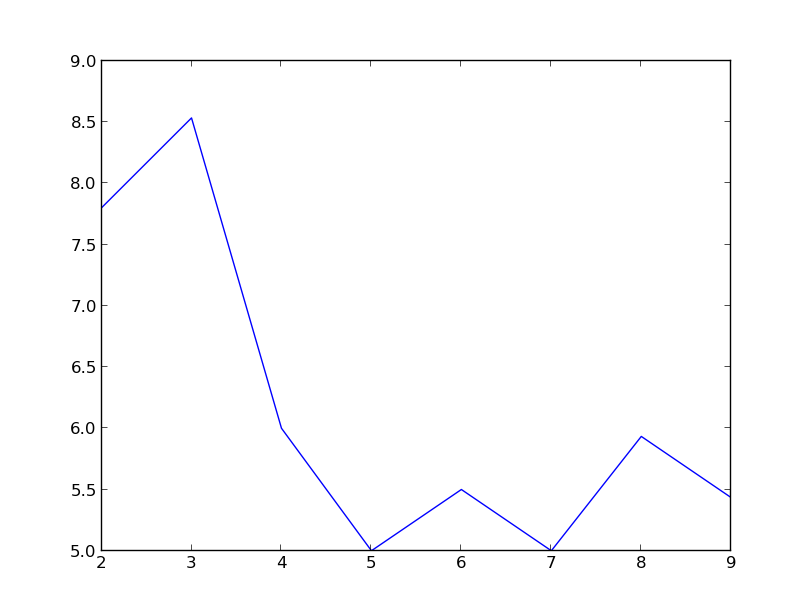
\includegraphics[scale=0.38]{imgs/scalabilityv1.png}
	\captionof{figure}{\textit{Master} using \texttt{MPI\_Recv}, single-core processing: execution time in order to the number of nodes.}
	\label{fig:mpi-recv-exec-time-by-cores}
\end{center}

\begin{center}
	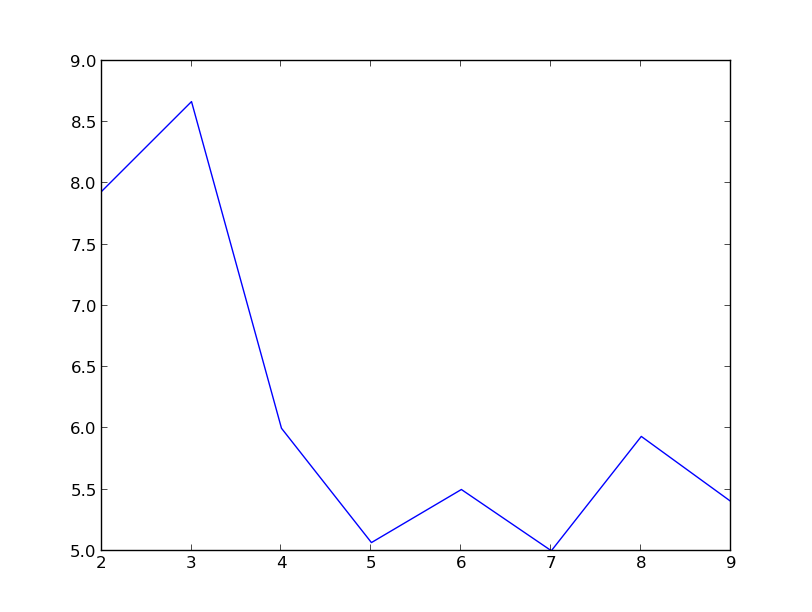
\includegraphics[scale=0.38]{imgs/scalabilityv2.png}
	\captionof{figure}{\textit{Master} using \texttt{MPI\_Irecv}, single-core processing: execution time in order to the number of nodes.}
	\label{fig:mpi-irecv-exec-time-by-cores}
\end{center}

\indent \indent Para as duas últimas soluções não existem gráficos para cada número de \textit{nodes}; no entanto, para as soluções com \texttt{OMP tasks} o tempo rondou os $6300ms$, enquanto que com \texttt{pthread\_create} o tempo demorado rondou aproximadamente os $6200$ para 9 máquinas; a solução \textit{single thread} de Irecv obteve $5800ms$ em média, com o seu melhor resultado de $\mathbf{5000ms}$ (melhor global) para 5 máquinas (isto é, 4 \textit{slaves}.

Quanto às duas abordagens \textit{multi-threaded}, o seu resultado foi pior do que as abordagens \textit{single-core} do \textit{master}; isto prende-se com o \textit{overhead} de criação de \texttt{threads} a cada request, da alocação, cópia e libertação de memória. Consideramos que esta abordagem beneficiaria da implementação de um esquema produtor/consumidor, de forma a usufruir dos dois \textit{cores} sem este overhead.

Antes de mais, notar que a diferença não se fez notar, uma vez que a utilização de \texttt{MPI\_Irecv} desceu ligeiramente a média de execução, mas mantendo a curva geral.

A análise que se segue prende-se à anormalia observada: \textit{runs} com número par de \textit{nodes}, ou seja, número ímpar de \textit{slaves}, obtêm piores resultados que os outros. Ainda que a diferença pudesse apenas estar relacionada com a discrepância na divisão das tarefas entre nós, tal não parece justificar a magnitude da diferença de performance. Uma vez que, durante a execução dos \textit{runs} dois dos 9 nós realçavam-se por demorar ligeiramente mais tempo que os outros, é possível que possa estar relacionado com os nós em utilização, uma vez que esta é uma solução virtualizada, o que não garante contenção total; de referir que a virtualização não se prende apenas ao nível de CPU e memória, mas mesmo ao nível do sistema de ficheiros (que, como mencionado anteriormente, apresentou algumas \textit{particularidades}).

A principal justificação, no entanto, para um ganho desta magnitude prende-se com o tempo gasto na comunicação entre máquinas, que faz com que não se rentabilizem os 2 \texttt{cores} das 9 máquinas. Utilizando os tempos já apresentados sobre o tempo de execução de um oitavo das transacções, obtém-se o valor de, aproximadamente, $1500ms$ para o tempo dispendido em comunicação entre processos (comparando com a versão \texttt{MPI\_Irecv}; com a versão \texttt{MPI\_Recv} são dispendidos $2845ms$\footnote{Este valor, ao contrário do relativo ao \texttt{MPI\_Recv}, foi medido envolvendo todas as chamadas à função com medições de tempo, e somando para obter um valor total; apesar de não medir com precisão o tempo de recepção, usamo-lo como forma de comparação.}). Parece-nos assim que o ganho foi considerável e que o \textit{overhead} em comunicação é \textit{adequado} à dimensão do problema.

De referir que os melhores runs ocorreram com 5 máquinas, onde se obtém um valor médio de $5000ms$ para a execução do programa. Assim, com 5 máquinas de 2 \textit{cores} de 2Ghz conseguimos obter a performance de uma máquina de 6 \textit{cores}.

\clearpage

\section{Conclusions}
\indent \indent Com as abordagens tomadas concluímos que, apesar do paradigma de programação exigido pelo \textit{Grid Computing} ser relativamente difícil de fazer \textit{debug}, torna-se fácil criar sistemas escaláveis a dezenas de máquinas com pequenas modificações no código. As preocupações devem recair (e recaíram) sobre as quantidades de dados trocadas na rede, sobre uma boa definição de uma cadeia de comando e de papéis para cada computador, de forma a minimizar os \textit{bottleneck}s.

Uma das abordagens que se pretendia ter aborado era a distribuição de trabalho por parte do \textit{master}, mas infelizmente não foi possível. Com a quantidade de dados que o \textit{master} teria que enviar e receber, era possível que tal obtesse pior performance; no entanto, dada o \textit{setup} da solução (comunicação de alta velocidade), é possível que os resultados fossem surpreendemente melhores.

Concluímos também que as variações entre \texttt{MPI\_Recv} e \texttt{MPI\_Irecv} são supérfluas, uma vez o \textit{master} consome a maior parte do seu tempo no processamento e não na recepção; acreditamos que se fizessem sentir que tivesse sido implementada um esquema de \textit{producer}/\textit{consumer} onde uma segunda \texttt{thread} do \textit{master} processasse os pedidos.
\clearpage
\end{document}